\subsection{Problem Formulation}\label{sec:cloud:data_centers:problem_formulation}

A widely used data center architecture is the three-tier architecture shown in \reffig{fig:sec:cloud:data_centers:problem_formulation:3-tier_datacenter}.
The upper two layers of the architecture are responsible for distributing the traffic and consist of layer 3 switches where each switch has a backup switch.
In this paper, we focus on the edge layer and here on a single \gls{POD}.
A \gls{POD} consists of a number of servers connected over top of rack switches to an aggregation switch.

\begin{figure}
  \centering
  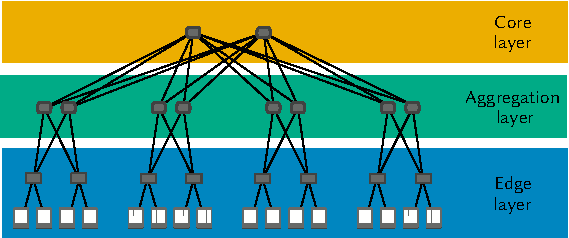
\includegraphics{cloud/data_centers/problem_formulation/figures/architecture}
  \caption{Three-tier data center architecture}
  \label{fig:sec:cloud:data_centers:problem_formulation:3-tier_datacenter}
\end{figure}


We assume, that new jobs entering the system arrive with exponentially distributed inter-arrival time.
When a job in form of a packet arrives at the \gls{POD}, it is forwarded to an idle server.
If no idle server is available, the job is queued.
Once a server finishes processing its current job, it picks another one from the queue.

Our goal is now to evaluate how much power is consumed in a data center and how much can be saved when servers, not processing any job, are switched off.
Therefore, we developed two different data center models.
The first model, the \emph{default data center}, consists of two-state servers only which are either \emph{busy} or \emph{idle}, as shown in \reffig{fig:sec:cloud:data_centers:problem_formulation:servers:two_state}) 
For the second model, a more \emph{energy-efficient data center}, a subset of the servers may additionally be switched on and \emph{off} on demand, shown in \reffig{fig:sec:cloud:data_centers:problem_formulation:servers:three_state} as recommended in~\cite{EPA2007}.

\begin{figure}
	\begin{subfigure}[b]{\textwidth}
	\centering
	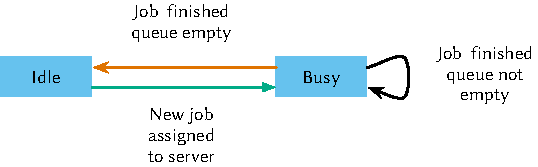
\includegraphics{cloud/data_centers/problem_formulation/figures/idle_busy}
	\caption{2-state server model}\label{fig:sec:cloud:data_centers:problem_formulation:servers:two_state}
	\end{subfigure} 
	\begin{subfigure}[b]{\textwidth}
	\centering
	\includegraphics{cloud/data_centers/problem_formulation/figures/idle_busy_offs}
	\caption{3-state model of a reserved server}\label{fig:sec:cloud:data_centers:problem_formulation:three_state}
	\end{subfigure}

	\caption{CPower state transition on a per server level}\label{fig:sec:cloud:data_centers:problem_formulation:servers}
\end{figure}
